%$$$$$$$$$$$$$$$$$$$$$$$$$$$$$$$$$$$$$$$$$$$$$$$$$$$$$$$$$$$$$$$$$$$$$$$$$$$$$$$$
% Paragraph 3: Scalable Data Structure and Lock에 대한 연구
%$$$$$$$$$$$$$$$$$$$$$$$$$$$$$$$$$$$$$$$$$$$$$$$$$$$$$$$$$$$$$$$$$$$$$$$$$$$$$$$$
\newpage
\section{확장성 있는 락 연구}
\label{sec:lockrelated}

%$$$$$$$$$$$$$$$$$$$$$$$$$$$$$$$$$$$$$$$$$$$$$$$$$$$$$$$$$$$$$$$$$$$$$$$$$$$$$$$$
%Paragraph : 기본적인 락에 대한 이야기와 확장성 있는 락의 필요성 
%$$$$$$$$$$$$$$$$$$$$$$$$$$$$$$$$$$$$$$$$$$$$$$$$$$$$$$$$$$$$$$$$$$$$$$$$$$$$$$$$
락의 기본적인 목적은 여러 스레드들을 안전하고 올바르게 동작하도록 만들어주는 방법이다.
이처럼 여러 스레드를 안전하게 동작시켜주기 위해, 락은 하드웨어 동기화 명령들(CAS,
fetch-and-add, SWAP 등)을 이용하여 구현되어 왔다. 
기본적으로 락의 구현은 코어들과 램(RAM)간에는 공유하는 버스가 있고, 이러한 버스를 이용하여 원자적으로 
처리하기 위해 하드웨어 동기화 명령을 이용한다. 
예를 들어 x86 시스템 같은 경우 하드웨어 동기화 명령인 \code{xchg} 명령어를 통해 쉽게 락을 구현할 수 있다.
하지만 실제 시스템은 보다 더 복잡한 구조를 가지게 되는데, 
복잡한 이유는 중간에 캐시 메모리와 일관성을 유지하기 위한 캐시 일관성 프로토콜 때문에 발생하는 문제를 
해결해야 하며, 또한 매니코어 NUMA 구조에 최적화 되도록 구현되야 하기 때문이다.


%$$$$$$$$$$$$$$$$$$$$$$$$$$$$$$$$$$$$$$$$$$$$$$$$$$$$$$$$$$$$$$$$$$$$$$$$$$$$$$$$
%Paragraph : 리눅스 락 구현에 대한 이야기
%$$$$$$$$$$$$$$$$$$$$$$$$$$$$$$$$$$$$$$$$$$$$$$$$$$$$$$$$$$$$$$$$$$$$$$$$$$$$$$$$
전통적으로 락의 프리미티브(Primitive)들은 두 종류로 구현되어 왔다.
하나는 바쁜대기(Busy-waiting) 방법과 다른 하나는 슬리핑(Sleeping) 또는 블락킹(Blocking) 방법으로 구현된다.
만약 락을 잡고 있는 시간이 적을 때는 바쁜대기(Busy-waiting) 방법을 사용한다. 
이 방법은 락이 풀릴 때까지 전역 변수를 CAS연산을 사용하여 반복적으로 전역 변수를 읽음으로 구현된다.
이것은 블락킹 방법의 문제점인 블락킹 오버헤드(스케줄링 오버헤드) 줄일 수 있으나, 
수행도중 CPU를 계속 사용함에 따라 다른 스레드들이 CPU를 점유하지 못하는 문제가 있다.
다른 방법인 블락킹 락은 락이 걸린동안 다른 스레드들을 동작시킬 수 있는 장점이 있으나, 
스케줄러의 스레드관리에 의존적이고 스케줄링 정책에 의해 락의 공정성등에 영향을 준다.

%$$$$$$$$$$$$$$$$$$$$$$$$$$$$$$$$$$$$$$$$$$$$$$$$$$$$$$$$$$$$$$$$$$$$$$$$$$$$$$$$
%Paragraph : 락과 확장성에 대한 이야기
%$$$$$$$$$$$$$$$$$$$$$$$$$$$$$$$$$$$$$$$$$$$$$$$$$$$$$$$$$$$$$$$$$$$$$$$$$$$$$$$$
최근 운영체제는 이 두가지 방법을 혼합하여 사용한다. 
최근 리눅스 커널의 블락킹 락은 \code{fastpath, optimistic spinning, slowpath}로 구현된 3가지의
락을 혼합하여 구현한다~\cite{Bueso2014STP}.
예를 들어 커널의 \code{rw\_semaphore}(reader-writer semaphore)는 아래와 같이 3가지 상태로 구현된다.
\begin{itemize}
\item \textbf{fastpath.} 아무도 락을 안잡고 있을 때, 원자적인 명령어(\code{fetch\_and\_add})를 이용하여
카운터를 수정하고 락과 함께 반환하는 부분이다.
\item \textbf{optimistic spinning.} 다른 스레드가 락을 잡고 있어서 기다려야 하는 상황이다.
Optimistic Spinning을 수행하는 이유는 락 경합에 발생하는 대기 시간이 대부분 짧다는 것이다.
따라서 이러한 상황에 대해서 블락킹 오버헤드를 줄이기 위해 바쁜대기(busy-waiting) 방법으로 수행한다. 
또한 최근에는 모든 코어가 같은 전역 변수를 읽을 경우 많은 캐시 일관성 트래픽이 발생하므로, 
락을 걸 코어에 등록하고 기다리는 코어에서는 해당 CPU의 로컬 변수만 주기적으로 확인하는 
큐 기반 락(MCS 기반 락)으로 구현한다. 
\item \textbf{slowpath.} 만약 락을 잡고 있는 시간이 길어지면, 대기 큐에 집어 넣고 슬립(Sleep)을 수행하는 블락킹 
락을 수행한다. 
\end{itemize}
이와 같이 이러한 하이브리드한 슬리핑 락은 많은 성능 향상을 보인다. 


%$$$$$$$$$$$$$$$$$$$$$$$$$$$$$$$$$$$$$$$$$$$$$$$$$$$$$$$$$$$$$$$$$$$$$$$$$$$$$$$$
%Paragraph :   atomic instructions 이야기
%$$$$$$$$$$$$$$$$$$$$$$$$$$$$$$$$$$$$$$$$$$$$$$$$$$$$$$$$$$$$$$$$$$$$$$$$$$$$$$$$



%$$$$$$$$$$$$$$$$$$$$$$$$$$$$$$$$$$$$$$$$$$$$$$$$$$$$$$$$$$$$$$$$$$$$$$$$$$$$$$$$
%Paragraph :   ts, ticket lock 이야기
%$$$$$$$$$$$$$$$$$$$$$$$$$$$$$$$$$$$$$$$$$$$$$$$$$$$$$$$$$$$$$$$$$$$$$$$$$$$$$$$$


%$$$$$$$$$$$$$$$$$$$$$$$$$$$$$$$$$$$$$$$$$$$$$$$$$$$$$$$$$$$$$$$$$$$$$$$$$$$$$$$$
%Paragraph : 락과 확장성 정리
%$$$$$$$$$$$$$$$$$$$$$$$$$$$$$$$$$$$$$$$$$$$$$$$$$$$$$$$$$$$$$$$$$$$$$$$$$$$$$$$$
이와 같이 확장성을 위해 락과 관련한 병렬 처리에서 고려해야 할 사항 정리하면,
기본적으로 락으로 보호해야 할 임계 영역(Critical Region)의 길이을 최대한 짧도록 해야하고, 
락 자체가 가지고 있는 오버헤드도 또한 고려해야 할 사항이다. 
또한 락의 세분화(Granularity) 정도에 따라 Find-grained 락을 사용할지 Coarse-grained 락을 사용해야 할지 
고려해야한다.

다음으로, 읽기-쓰기 비율을 고려하여 읽기가 많은 경우에는 읽기-쓰기 락을 사용하고,
읽기가 많으며 오래된(stale) 데이터도 허락되는 자료구조에서는 RCU 같은 동기화 기법을 사용해야 한다.  
또한 약간의 공정성(Fairness) 손해보더라도 NUMA 기반에서 확장성을 높이는 방법도 고려해야 한다.
마지막으로 최근 락에 대해서 중요한 요소로 생각하고 있는 캐시 일관성 때문에 발생하는 
오버헤드를 고려해야 한다. 

%~\cite{MellorCrummey1991MCS}~\cite{Magnusson1994QLC},
% ~\cite{Wang2016BeMyGuest}, ~\cite{Scott2013SS}
%~\cite{Bueso2014MCS}~\cite{Bueso2015STP}

%

%~\cite{Hendler2010FC}~\cite{Fatourou2012RCS}~\cite{Delegation2014}

이러한 고려사항들을 적용하여 확장성있는 락에 대한 연구는 큐 기반의
락과 계층적 락 그리고 위임하는 방법(Delegation Techniques)들이 연구되고 있다. 

\subsection{큐 기반의 락(Queued Lock)}
%\subsubsection{MCS}
%$$$$$$$$$$$$$$$$$$$$$$$$$$$$$$$$$$$$$$$$$$$$$$$$$$$$$$$$$$$$$$$$$$$$$$$$$$$$$$$$
%Paragraph :   MCS 이야기
%$$$$$$$$$$$$$$$$$$$$$$$$$$$$$$$$$$$$$$$$$$$$$$$$$$$$$$$$$$$$$$$$$$$$$$$$$$$$$$$$
모든 코어가 바라보는 전역 변수를 사용하기 때문에 발생하는 캐시 일관성 트래픽 문제는 
락 내부에서도 발생한다. 
그 동안 락의 구현은 하나의 전역변수를 대상으로 원자적 명령을 이용하여 구현하였다. 
따라서 자연히 캐시 일관성 트래픽 문제가 발생하였는데, 이것을 해결하는 방법이 큐 기반의 락
~\cite{MellorCrummey1991MCS}~\cite{Magnusson1994QLC}~\cite{Wang2016BeMyGuest}~\cite{Scott2013SS}
~\cite{Bueso2014MCS}을 이용하는 것이다. 

락 때문에 발생하는 캐시 일관성 문제를 해결하기 위한 가장 쉬운 접근하는 방법은 각 
코어가 모두 다른 캐시 라인의 데이터를 가지고 스핀을 하면 쉽게 해결이 된다.
즉 각각의 코어가 \textit{read-only} 스핀을 하고, 반환 하는 스레드가 명시적으로 해당 코어의 캐시 라인의 데이터를 
원자적 명령을 이용하여 락을 반환하는 것이다. 
이러한 방법의 문제점은 공간적인 문제가 있다. 
즉 모든 락이 모든 코어의 중복되지 않도록 캐시 라인 데이터를 위한 공간을 확보해야 한다는 것이다.
이것은 현실적으로 메모리 낭비가 심히다.
이러한 문제를 해결한 것이 CLH 큐 기반 락이다. 
이러한 배열 기반으로 모든 코어가 같은 전역 변수를 바라 보며 스핀하지 않고, 
각자의 로컬 변수를 바라 보며 스핀하도록 하여, 확장성을 향상 시킨 방법이다. 
즉 기존 많은 공간(락 * 스레드 수)이 필요할 것을 적은 공간(락 + 스레드 수)로도 구현이 가능하게 되었다.

또한 배열 기반의 메모리 낭비를 더 줄이기 위해 MCS 락이 개발되었다. 
각 락에 대한 정보를 링크드 리스트로 보관하자는 것이 기본적인 아이디어이고, 
이것은 하나의 스레드는 반드시 하나의 락만 기다린다는 아이디어를 활용하여 리스트로 기다리는 
스레드들을 관리하였다. 
 
%$$$$$$$$$$$$$$$$$$$$$$$$$$$$$$$$$$$$$$$$$$$$$$$$$$$$$$$$$$$$$$$$$$$$$$$$$$$$$$$$
%Paragraph 2: scalable locks의 성능에 대한 이야
%$$$$$$$$$$$$$$$$$$$$$$$$$$$$$$$$$$$$$$$$$$$$$$$$$$$$$$$$$$$$$$$$$$$$$$$$$$$$$$$$
MCS 락의 성능은 적은 코어 즉 코어 수일 경우 티켓 락이 더 좋은 성능을 보이지만, 
코어 수가 많아 질수록 MCS 락은 좋은 성능을 보인다. 
이처럼 락을 확장성 있는 락을 사용하면, 락 때문에 발생하는 확장성 문제 즉 성능이 갑자기 떨어지는 현상을 
막을 수 있으나, 근본적으로 확장성 있는 시스템을 구축하려면 반드시 임계 영역의 길이를 줄여야한다.
이러한 장점을 받아들여, 리눅스 커널도 처음에는 티켓 락 기반의 스핀락을 사용했으나, 
2013년 이후 티켓-스핀락을 MCS-스픽락으로 변경하였다. 
엄밀하게 말하면 리눅스 커널은 MCS의 기본적인 자료구조 사이즈가 크기 때문에, 커널은 MCS 락을 커널 크기에 
맞도록 수정하여 사용한다. 
결국 2016년 부터는  리눅스 커널에서 티켓 락 기반의 스핀락은 사라지게 되었다~\cite{ticket}.
 
\subsection{계층적 락}

%$$$$$$$$$$$$$$$$$$$$$$$$$$$$$$$$$$$$$$$$$$$$$$$$$$$$$$$$$$$$$$$$$$$$$$$$$$$$$$$$
%Paragraph 2: 계층적 락
%$$$$$$$$$$$$$$$$$$$$$$$$$$$$$$$$$$$$$$$$$$$$$$$$$$$$$$$$$$$$$$$$$$$$$$$$$$$$$$$$
계층적인 락~\cite{Radovic2003HBL}~\cite{Chabbi2016CLL}~\cite{Luchangco2006HCQ}
~\cite{Chabbi2015HPL}들의 공통적인 목적은 스케일이 큰 NUMA 환경에서 확장성을 높이는 공통적인 목적을 가진다.  
특히 NUMA 환경에서는 원격 소켓의 데이터를 접근하는 것 때문에 성능이 저하되는 문제를,
소켓 단위로 락의 이주(Migration)을 줄여서 향상시키는 방법이다.
또한 이러한 계층적 락에 대한 연구는 여러 소켓을 전역 락과 소켓 안에서 관리하는
지역 락을 따로 두어 약간의 공정성(Fairness)를 손해보더라도, 
NUMA 노드의 지역성을 향상 시켜서 성능을 향상시키는 방법이다.

\subsection{Delegation techniques}

\subsubsection{Flat Combining}

%$$$$$$$$$$$$$$$$$$$$$$$$$$$$$$$$$$$$$$$$$$$$$$$$$$$$$$$$$$$$$$$$$$$$$$$$$$$$$$$$
%Paragraph :   Flat Combining 이야기
%$$$$$$$$$$$$$$$$$$$$$$$$$$$$$$$$$$$$$$$$$$$$$$$$$$$$$$$$$$$$$$$$$$$$$$$$$$$$$$$$
\code{Flat combining}(FC)~\cite{Hendler2010FC}는 여러 코어에서 캐시 일관성 트래픽 문제를 발생시키는 
락을 호출하면서 연산을 수행하는 것 보다, 하나의 코어에서 한 스레드가 해당 명령어들을 
모아서 하나의 전역 락을 사용하여 처리하는 것이 더 효율적이라는 것을 주장하는 논문이다.
그리고 이러한 철학을 하나의 동기화 기법으로 만든것 FC이다.
FC는 두 가지 장점을 가지는데 가장 먼저 FC는 락을 자주 수행하지 않으므로, 락에 의한 
캐시 일관성 트래픽이 상대적으로 덜 발생한다는 것이다.
다음으로 하나의 스레드에서 여러 읽기 쓰기 연산을 수행함에 따라, 캐시 지역성이 높아져서 
여러 스레드들이 직렬화 되어 수행한 방법보다 높은 성능을 가진다는 것이다. 

\begin{figure}[h!]
    \centering
    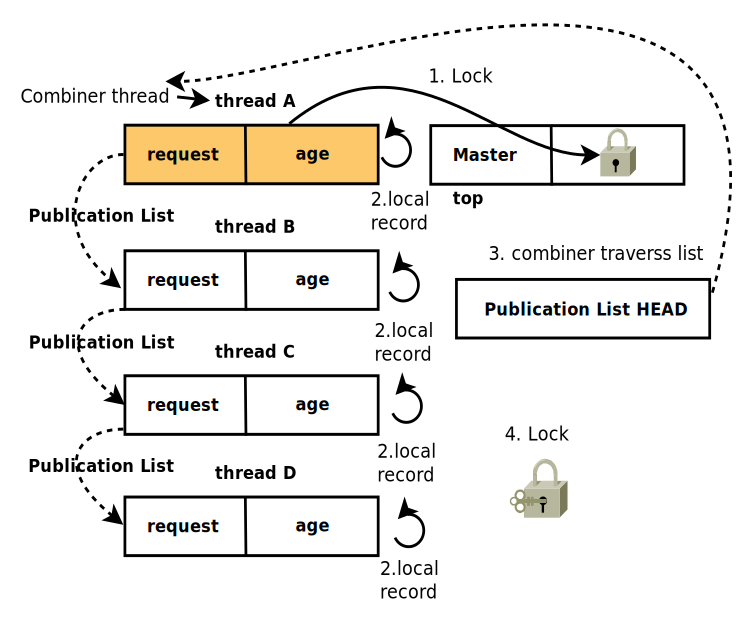
\includegraphics[width=1\textwidth]{fig/FC/FC}
    \caption{Flat combining 방법}
  \label{fig:FC}
\end{figure}

%$$$$$$$$$$$$$$$$$$$$$$$$$$$$$$$$$$$$$$$$$$$$$$$$$$$$$$$$$$$$$$$$$$$$$$$$$$$$$$$$
%Paragraph :   Flat Combining 알고리즘
%$$$$$$$$$$$$$$$$$$$$$$$$$$$$$$$$$$$$$$$$$$$$$$$$$$$$$$$$$$$$$$$$$$$$$$$$$$$$$$$$
그림~\ref{fig:FC}는 FC 알고리즘의 방법에 대해서 설명한다. 
먼저 자료구조에 대한 연산(예를 들어 스택같은 경우 \code{push} 또는 \code{pop})가 도착하면, 
처음 받은 스레드는 락을 걸고, 해당 명령어를 수행한다. 
동시에 다른 코어의 스레드들은 다른 명령어들을 수행하게 되는데, 각 코어의 스레드들은 
받은 연산들을 코어의 내부 변수에 요청 정보과 시간 정보(age)를 같이 저장 한다.
처음 받은 스레드의 연산이 끝나면 이때 부터 각 스레드에 저장된 연산들을 순회하면서 \code{combiner} 스레드가 
모든 연산들을 수행하고 마지막으로 락을 푼다.

\subsubsection{OpLog}
%$$$$$$$$$$$$$$$$$$$$$$$$$$$$$$$$$$$$$$$$$$$$$$$$$$$$$$$$$$$$$$$$$$$$$$$$$$$$$$$$
%Paragraph 2: OpLog 이야기
%$$$$$$$$$$$$$$$$$$$$$$$$$$$$$$$$$$$$$$$$$$$$$$$$$$$$$$$$$$$$$$$$$$$$$$$$$$$$$$$$

\begin{figure}[h]
    \centering
    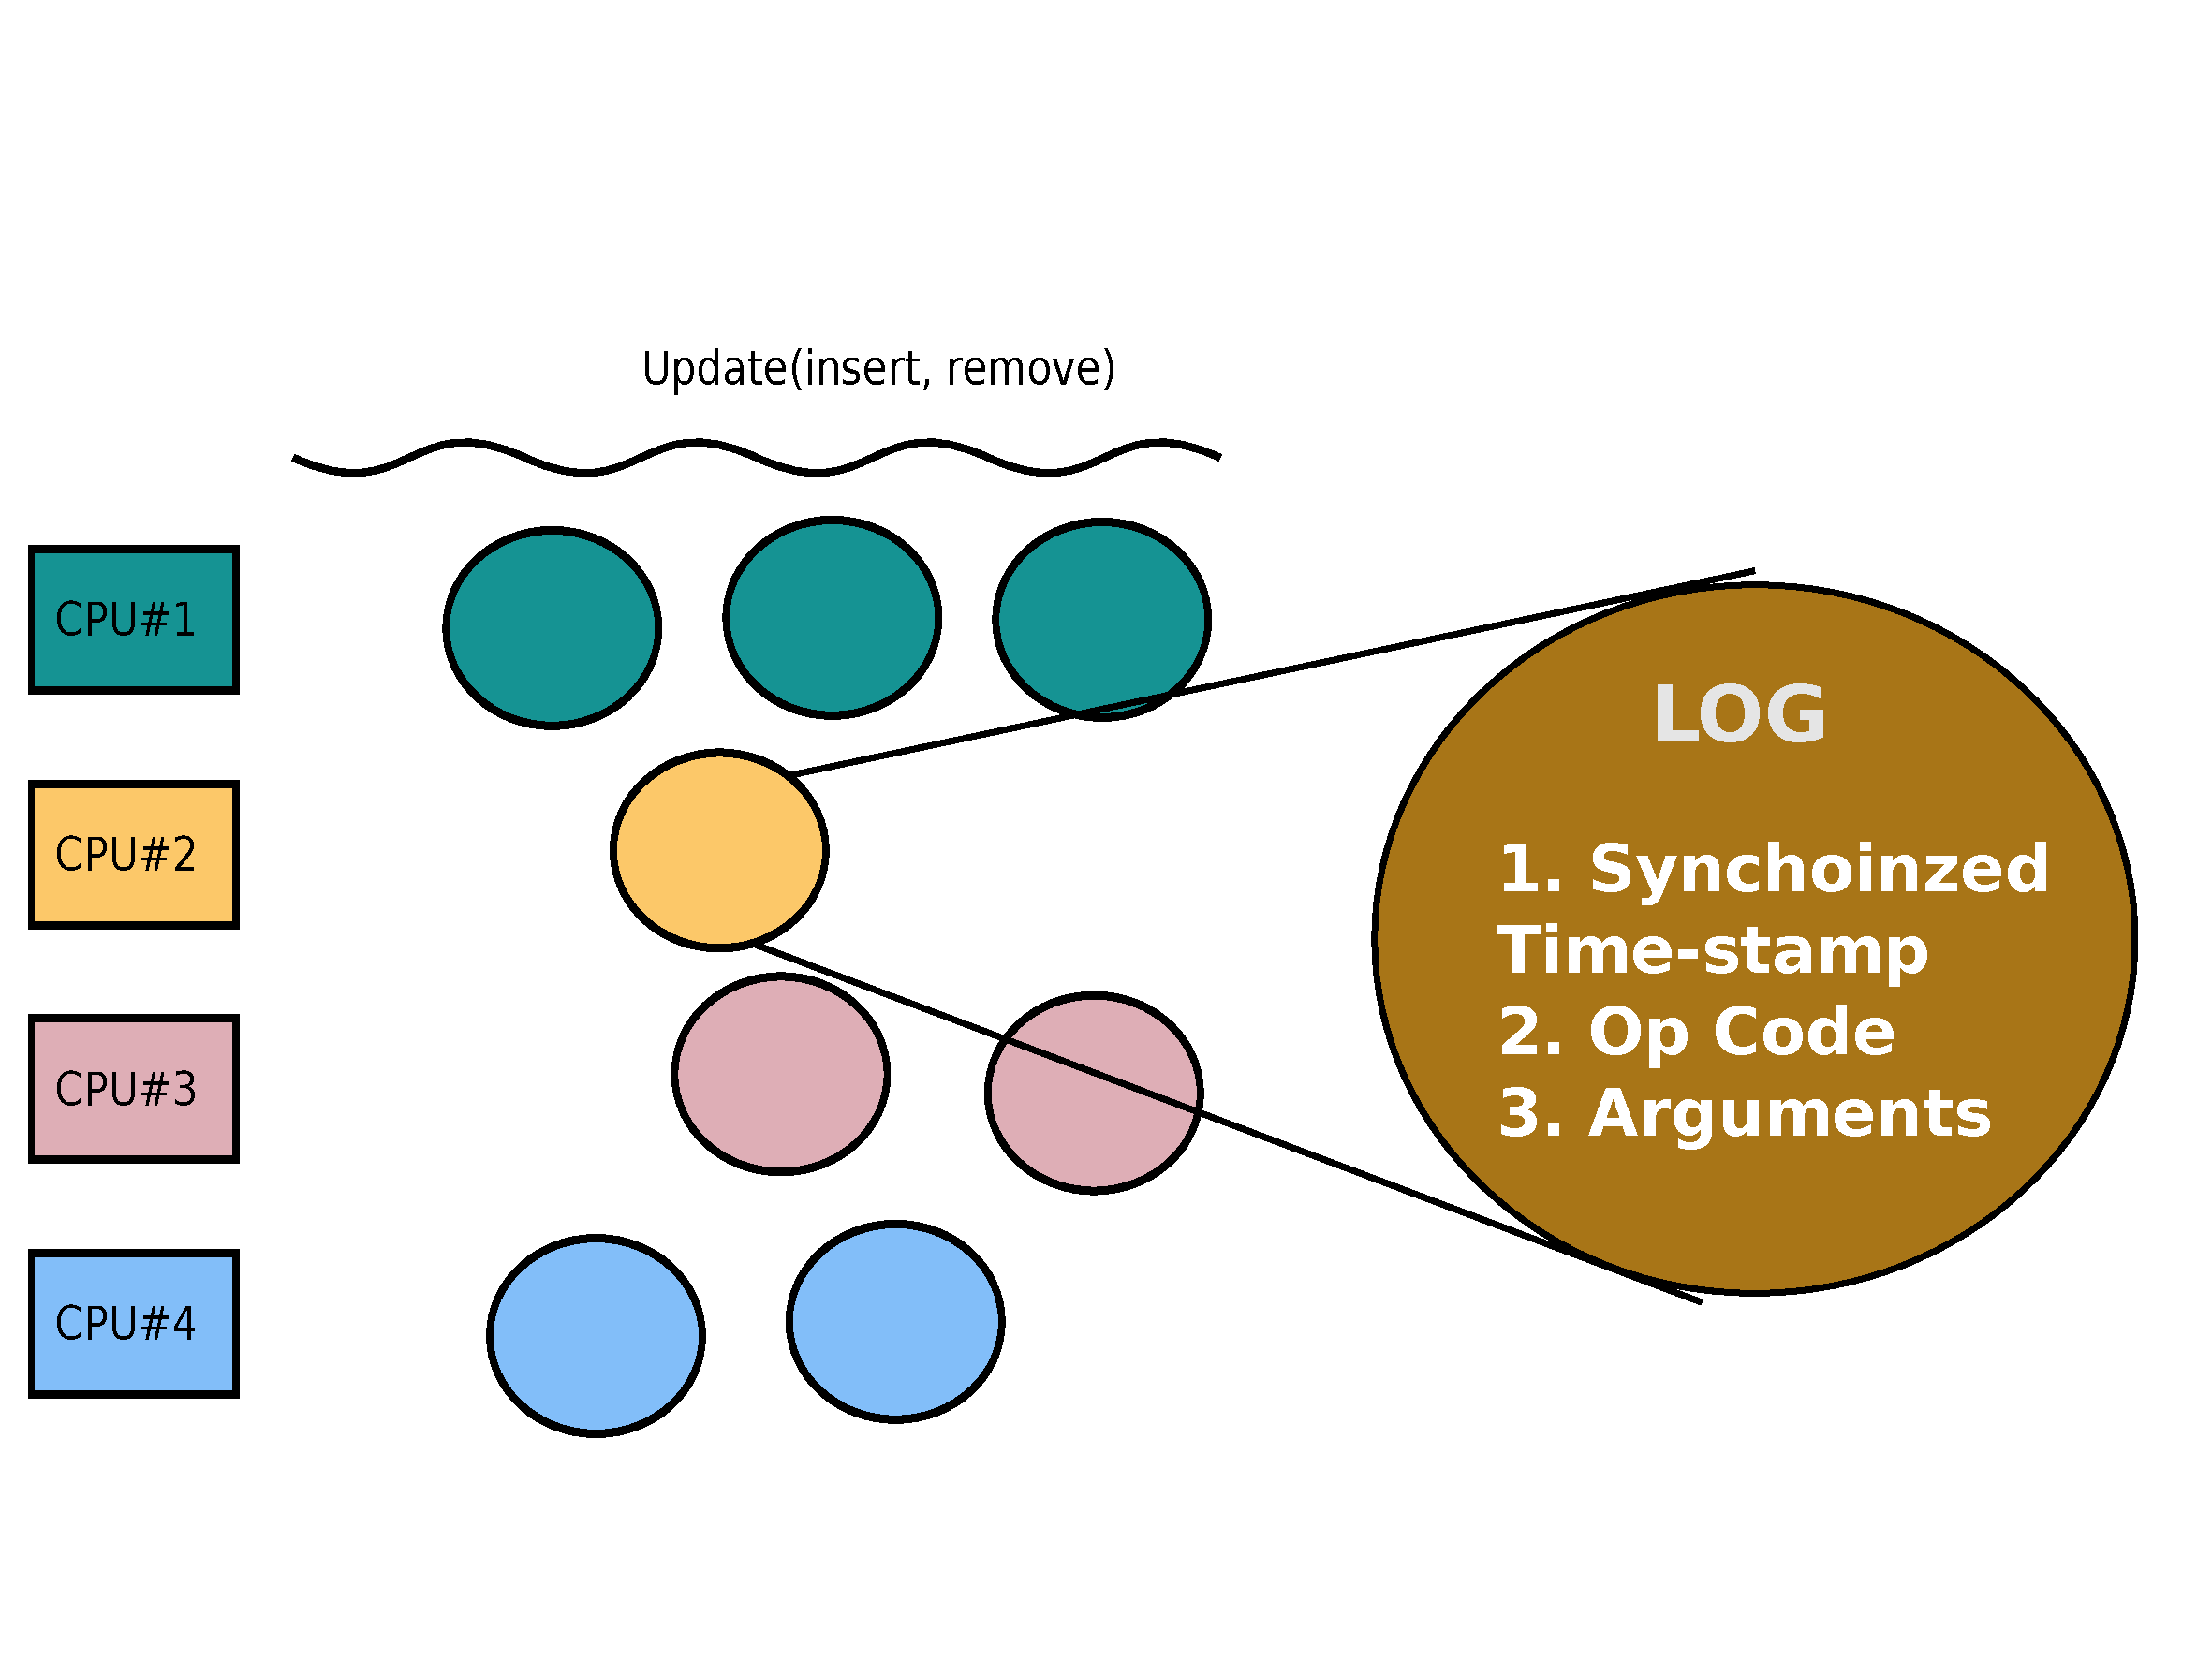
\includegraphics[width=0.8\textwidth]{fig/oplog_log}
    \caption{OpLog의 업데이트 방법}
  \label{fig:oplog}
\end{figure}

OpLog는 \code{read-mostly} 자료구조를 위한 RCU와 반대로 업데이트 비율이 \code{update-heavy} 한 
자료구조를 위해 만든 동기화 기법 중 하나이다.
업데이트가 많아질 경우, 락에 의해 문제가 생기는데, 기존 연구들의 해결방법들은 
CAS등을 사용하여 공유 데이터를 접근함에 따라, 이때 발생하는 캐시 일관성 트래픽에의해 
성능이 많이 떨어 진다는 것이다.
이러한 문제점을 해결하기 위한 방법 중 하나가 로그 기반으로 처리하는 것인데, OpLog는 이러한 로그 기반 
방법을 동기화된 타임스탬프 카운터를 이용하여 퍼코어에 로그를 저장함으로써 해결하였다. 
각 코어에 동기화된 타임스탬프와 함께 명령어를 로그로 저장을 한 다음, 읽기 연산이 수행되기 전에 
퍼코어에 저장된 로그를 타임스탬프 정보 함께 시간 순서대로 처리하는 방법이다.
그림~\ref{fig:oplog}는 각 코어에 저장된 로그 정보를 보여준다.
업데이트 명령어가 발생하면, 각 코어는 타임스탬프 정보, 연산 코드 그리고 연산을 처리하기 위한 
인자 값들을 함께 저장한다.

%$$$$$$$$$$$$$$$$$$$$$$$$$$$$$$$$$$$$$$$$$$$$$$$$$$$$$$$$$$$$$$$$$$$$$$$$$$$$$$$$
%Paragraph 2: OpLog의 타임 스탬프
%$$$$$$$$$$$$$$$$$$$$$$$$$$$$$$$$$$$$$$$$$$$$$$$$$$$$$$$$$$$$$$$$$$$$$$$$$$$$$$$$
OpLog는 동기화된 타임스탬프를 이용한다. 
하지만 여러 소켓으로 구성된 NUMA 시스템 같은 경우 소켓별로 \textit{clock source}가 다르므로, 
아직까지 동기화 타임스탬프는 하드웨어적으로 지원하지 않는 문제가 있다.
OpLog는 동기화 타임스태프 카운터가 있다는 것을 가정하여, 임시로 소프트웨어 동기화된 
타임스탬프 카운터를 구현하여 만든 동기화 기법이다. 
OpLog는 최근까지 하드웨어적인 동기화 타임스탬프 카운터가 지원하지 않으므로 
현실적으로 적용되는데 문제가 있다.


